\clearpage

\section{Riemannin ikkuna}

\begin{wrapfigure}{r}{0.4\textwidth}
  \begin{center}
    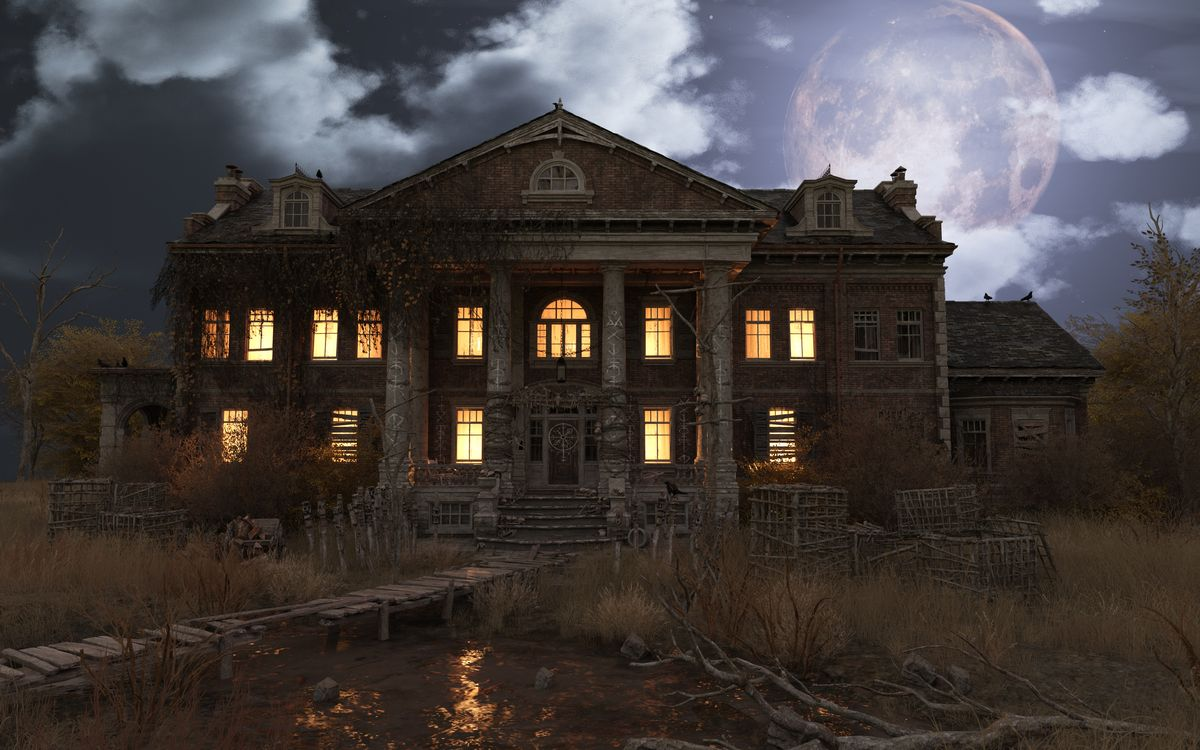
\includegraphics[width=0.38\textwidth]{kuvat/riemann_kartano.jpg}
  \end{center}
\end{wrapfigure}

Luuranko Riemann on rakentamassa itselleen suurta ja pelottavaa kartanoa. Hän haluaa kartanon julkisivulle näyttävän ikkunan. Riemann päättää tehdän ikkunasta parabelin muotoisen. Ikkunan korkeudeksi tulee $2 \ \text{m}$ ja leveydeksi $4 \ \text{m}$.


Paljonko Riemann tarvitsee lasia ikkunan valmistamiseen?

Lisätehtävä: Paljonko puuta ikkunan kehyksiin tarvitaan?